\chapter{Wave polarization}\label{lec:lec23}
Here in this chapter we will be investigating one of the very important aspect of electromagnetism called \textbf{Wave Polarization}. Wave polarization is the behavior of electric field vector as a function of time at any point in space.

For a transverse electromagnetic wave, the direction of the electric and magnetic field are perpendicular to each other and also, they are perpendicular to the direction of propagation of the electromagnetic wave. However, the direction of the electric and magnetic field vectors can change as a function of time and that phenomenon is captured by what is called \textbf{Wave Polarization}.

Any electric field vectors can be described as a combination of two perpendicular electric field vectors; i.e the x-oriented and y-oriented field vectors. 
\begin{figure}[h]
\centering
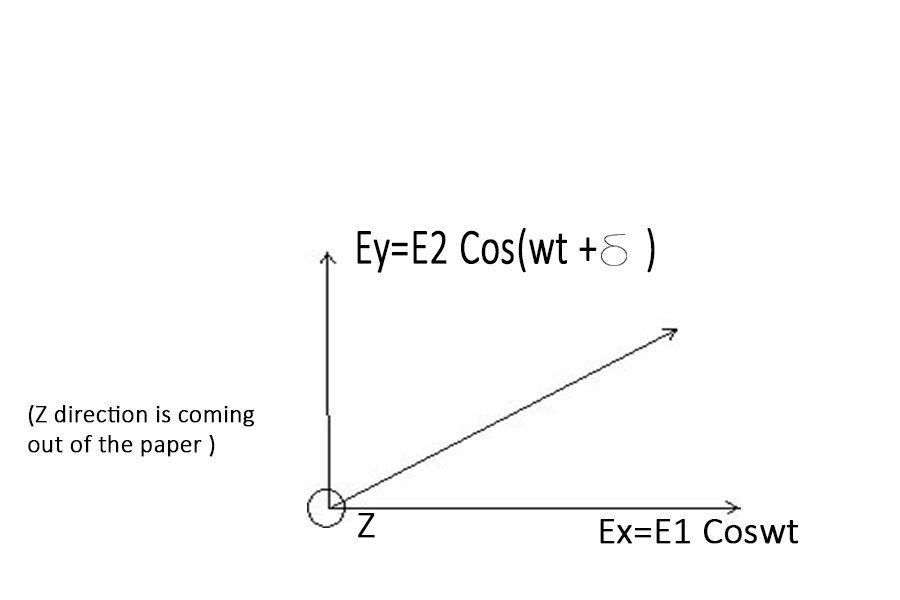
\includegraphics[width=.8\linewidth]{./graphics/electricfield}
\caption{electric field vector}
\end{figure}

In the analysis of the wave propagation, we assume that the wave is propagating in the positive Z direction (z-direction is coming out of the paper). And the two electric fields are sinusoidally varying as a function of time, with different amplitudes and phase difference between them.	

\section{The electric field vectors} 
From the diagram in figure 23.1, we can see that;
\begin{equation}
E_y = E_2 [\cos(\omega t + \delta)]
\end{equation}
\begin{equation}
E_x = E_1 \cos(\omega t)
\end{equation}
At any instant of time,the total electric field is the vector sum of the two electric  fields and from the graph,we can obtain the following;
\begin{equation}
\cos {\omega t} = \frac {E_x}{E_1} 
\end{equation}
from Pythagoras Theorem ($hyp^2$ = $opp^2$ + $adj^2$) and $ \cos x = \frac{opp}{hyp}$,also $\sin^2 x + \cos^2 x = 1$ then $\sin x = \sqrt{1-\cos^ 2x}$
\begin{equation}
\sin {\omega t} = \sqrt{1 - \frac{E_{x}^2}{E_{1}^2}}
\end{equation}
If we are interested in the behavior of the electric field as a function of time, and the electric field is treated like an arrow, then the tip is varying as a function of time in the electric field amplitude space and that indicate the state of Polarization of the Electromagnetic wave. Essentially, we are looking for the locus of the electric field as a function of time,so we will eliminate time parameters from the two component and the following will be obtained;

Recall from figure 23.1; 
\begin{equation}
\cos{\omega t} = \frac{E_x}{E_1}
\end{equation}
\begin{equation}
\sin (\omega t) = \sqrt{1-\frac{E_{x}^2}{E_{1}^2}}
\end{equation}
\begin{equation}
E_y = E_2 [\cos(\omega t + \delta)]
\end{equation}
Recall from compound angle formula that; $\cos(A+B) = \cos(A)\cos(B) - \sin(A)\sin(B)$ 
\begin{equation}
E_y = E_2 [\cos(\omega t)\cos(\delta) -\sin(\omega t) \sin(\delta)]
\end{equation}
now we substitute the value of $\cos{\omega t}$ and $\sin{\omega t}$ into the above equation
\begin{equation}
\frac{E_y}{E_2} =[\frac{E_x}{E_1}\cos(\delta)-(\sqrt{1 - \frac{E_{x}^2}{E_{1}^2}})\sin(\delta)]
\end{equation}
Rearranging the equation and squaring both side,we will get;
\begin{equation}
{[\frac{E_x}{E_1}\cos{\delta}-\frac{E_y}{E_2}]}^2 = [1-\frac{E_{x}^2}{E_{1}^2}]\sin^2(\delta)
\end{equation}
Recall that ${(a-b)}^2$ = $(a^2-2ab+b^2)$, so the equation above becomes;
\begin{dmath}
\frac{E_{x}^2}{E_{1}^2}\cos^2{\delta}-2(\frac{E_{x}E_{y}}{E_{1}E_{2}}\cos{\delta}) + \frac{E_{y}^2}{E_{x}^2} = \sin^2(\delta)-\frac{E_{x}^2}{E_{1}^2}\sin^2(\delta)
\end{dmath}
Rearranging the above equation we will get;
\begin{equation}
\frac{E_{x}^2}{E_{1}^2}[\cos^2{\delta} + \sin ^2(\delta)] - 2[\frac{E_{x}E_{y}}{E_{1}E_{2}}\cos{\delta}] + \frac{E_{y}^2}{E_{x}^2} = \sin^2(\delta)
\end{equation}
Also recall that $ \sin^2{a} + \cos^2{a} =  1$

So the equation which the tip of the electric field vector draws is given by the equation.
\begin{equation}
\frac{E_{x}^2}{E_{1}^2} -2(\frac{E_{x}E_{y}}{E_{1}E_{2}})\cos\delta + \frac{E_{y}^2}{E_{2}^2} =\sin^2 \delta
\end{equation}

\section{General equation }
Generally,this equation is similar to the equation of an ellipse ($\frac{x^2}{a^2} + \frac{y^2}{b^2} = 1 $), the tip of the electric field vector draws an ellipse in the electric field amplitude space as a function of time, and it will rotate the number of frequency times in a second. Having two parameters now,there are specialized cases now that can be investigated.The two parameters are;
\begin{enumerate}[(i)]
\item The amplitudes of the electric fields
\item The phase difference between them
\end{enumerate}
Keeping in mind we are only interested in the shape that the tip of the electric field vectors draws as a function of time and the size does not matter; i.e the absolute value of the $ E_1 $ and $ E_2 $ does not matter as far as the state of polarization is concerned, what matters is the ratio of the two quantities and phase difference between $ E_x $ and $ E_y $.

\footnote{When these two parameters are changed what are the shapes that will be obtained or drawn. Let see the different cases.}So essentially for defining the state of polarization, the following  are required;
\begin{enumerate}[(i)] 
\item The ratio of $ E_2 $ and $ E_1 $
\item The phase difference between the $ E_x $ and $ E_y $, delta ($\delta)$.
\end{enumerate}

\subsection{Case 1: delta ($\delta $) is zero}
Substituting $\delta$ = 0, into the equation 23.13,we will get;
\begin{equation}
\frac{E_{x}^2}{E_{1}^2} -2(\frac{E_{x}E_{y}}{E_{1}E_{2}}) + \frac{E_{y}^2}{E_{2}^2} = 0
\end{equation}
Recall that ${(a - b)}^2 = (a^2 -2ab +b^2)$,then the the equation above becomes;
\begin{equation}
{(\frac{E_x}{E_1} - \frac{E_y}{E_2})}^2 = 0
\end{equation}
find the square root of both sides and make $ E_y $ the subject of formula, the equation becomes;

\begin{equation}
E_y = \frac{E_2}{E_1}E_x
\end{equation}

which is similar to the equation of a straight line (y = mx +c)
if $\delta$ = 0, then the tip of the electric field vector draws a straight line as a function of time and the ratio of $ E_2 $ to $ E_1 $ determines the slope of the line.
\begin{enumerate}[(i)]
\item If $ E_2 $ is zero, the slope becomes zero and the line becomes horizontal.
\item If $ E_1 $ is zero, the slope becomes infinite and the line becomes vertical.
\end{enumerate} 
In general, the line will be oriented between X and Y axis, and the slope will be given by ($ \tan^{-1}[\frac{E_2}{E_1}]$)

Since the tip of the electric field is now drawing a straight line, we call this polarization as linear polarization and the condition is that the phase difference between the two electric vectors should be zero (0).
\begin{figure}[h]
\centering
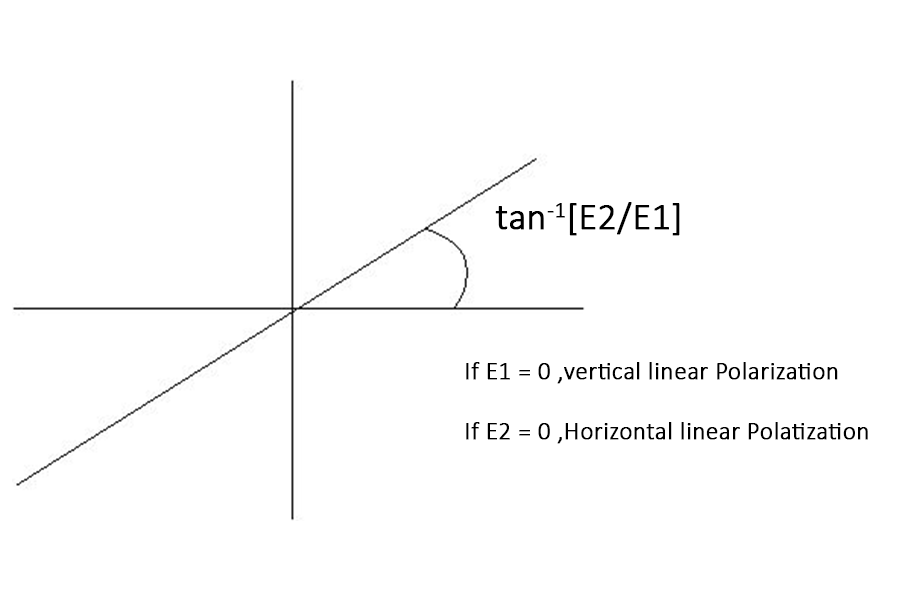
\includegraphics[width=.8\linewidth]{./graphics/electric2}
\caption{electric field vector}
\end{figure}

For a special case, where $  E_1=E_2 $, the line is at $ 45^{o}$ with respect to X axis.
Generally,if the phase difference between the electric field vectors is zero (0), we will always get a linear polarization. This is one of the special cases of the general ellipse.

\subsection{Case 2: $ E_1 = E_2 $ and $\delta = \pm \frac{\pi}{2}$}
When $\delta = \pm \frac{\pi}{2}$ is substituted into the general equation the following will be obtained.
\begin{equation}
\frac{E_{x}^2}{E_{1}^2} -2(\frac{E_{x}E_{y}}{E_{1}E_{2}})(0) + \frac{E_{y}^2}{E_{2}^2} = 1
\end{equation}
\begin{equation}
\frac{E_{x}^2}{E_{1}^2} + \frac{E_{y}^2}{E_{2}^2} = 1
\end{equation}
assuming that $ E_1 $ = $ E_2 $ = $ E_{o} $, cross multiply, then the equation becomes;
\begin{equation}
{E_{x}^2} + {E_{y}^2} = {E_{o}^2}
\end{equation}
This is similar to the equation of a circle $(x^2 + y^2 = r^2)$ the general equation of an ellipse is reduced to the equation of a circle. In this condition, the state of polarization is called \textbf{Circular polarization}.

whether  $\delta$ is $+\dfrac{\pi}{2}$  or  $-\dfrac{\pi}{2} $, the shape drawn is a circle but the way the shape is drawn is determined by the sign of $\delta$.

If the y component of the electric field leads, then we obtain a rotation in the clockwise direction, but if the y component lags, then we obtain a rotation in the anti-clockwise direction; i.e when $\delta$ is positive, and the observer is oriented in the direction of wave propagation, then we have a left-handed circular wave propagation. But, when $\delta$ is negative, and the observer is oriented in the direction of wave propagation, then we have a right-handed circular wave propagation.
\begin{enumerate}[(i)]
\item LH circular, $\delta$ is $ +\dfrac{\pi}{2}$ and $ E_1 = E_2$
\item RH circular, $\delta$ is $-\dfrac{\pi}{2}$ and $ E_1 = E_2$ 
\end{enumerate}
\begin{figure}[h]
\centering
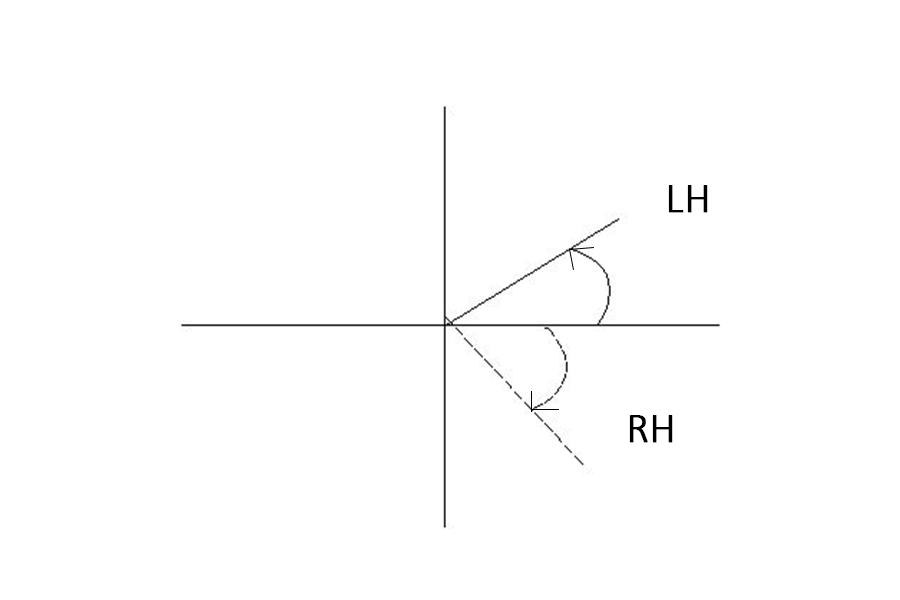
\includegraphics[width=.8\linewidth]{./graphics/fielddirect}
\caption{circular polarization}
\end{figure} 

So when we define the state of polarization, only the tip of the electric field does not completely describe the state of polarization, but combined with sense of direction gives the complete state of polarization

In a general case, when non of the condition is satisfied;i.e $ E_1 \neq E_2$, and $\delta\neq\dfrac{\pi}{2}$ or $ 0 $, in a third case.

\subsection{Case 3: \texorpdfstring{$E_1\neq E_2$}{E1≠E2} and \texorpdfstring{$\delta\neq\pm\frac{\pi}{2}$}{δ≠𝜆/2}}
Substituting the value of $\delta$ into equation 23.13, the equation becomes;
\begin{figure}[h]
\centering
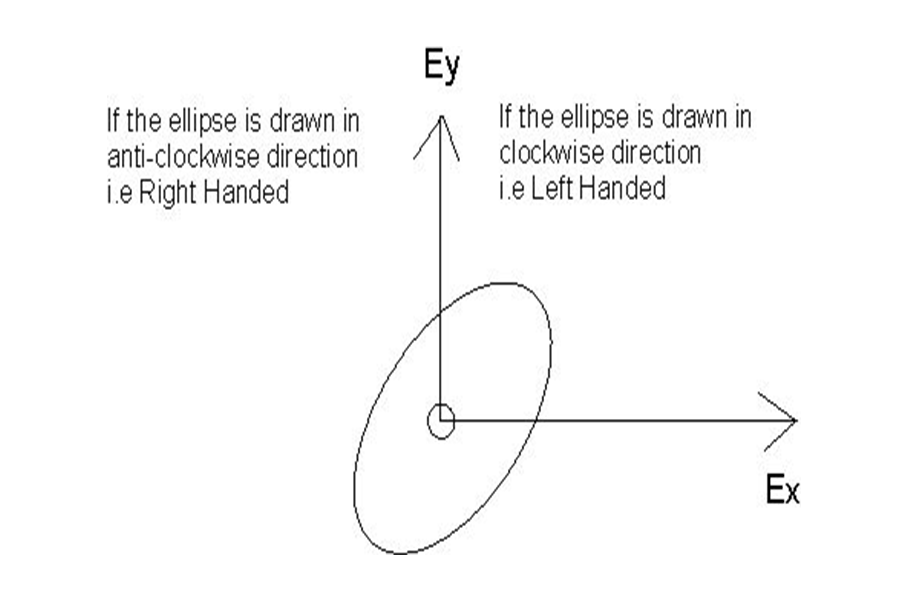
\includegraphics[width=.8\linewidth]{./graphics/ellipse}
\caption{elliptical polarization}
\end{figure}

\begin{equation}
\frac{E_{x}^2}{E_{1}^2} -2(\frac{E_{x}E_{y}}{E_{1}E_{2}})\cos\delta + \frac{E_{y}^2}{E_{2}^2} =\sin^2 \delta
\end{equation}

This equation is the same as the general equation (the elliptical equation). Elliptical polarization like we obtained earlier with circular polarization, also have it that;

Positive $\delta$ gives left-handed while a negative $\delta$ gives Right handed. The axis of the ellipse is at the origin i.e; along the major and minor axis of the ellipse.

\section{The Elliptical Polarization}
Here $E_1\neq E_2$ and $\delta = \pm \dfrac{\pi}{2} $. Substituting $\pm \delta$ into equation 23.13,the equation becomes;
\begin{equation}
\frac{E_{x}^2}{E_{1}^2} -2(\frac{E_{x}E_{y}}{E_{1}E_{2}})(0) + \frac{E_{y}^2}{E_{2}^2} = 1
\end{equation}
\begin{equation}
\frac{E_{x}^2}{E_{1}^2} + \frac{E_{y}^2}{E_{2}^2} = 1
\end{equation}
This is similar to the equation of an ellipse, ($\frac{x^2}{a^2}$ + $\frac{y^2}{b^2}$ = 1).
\begin{figure}[h]
\centering
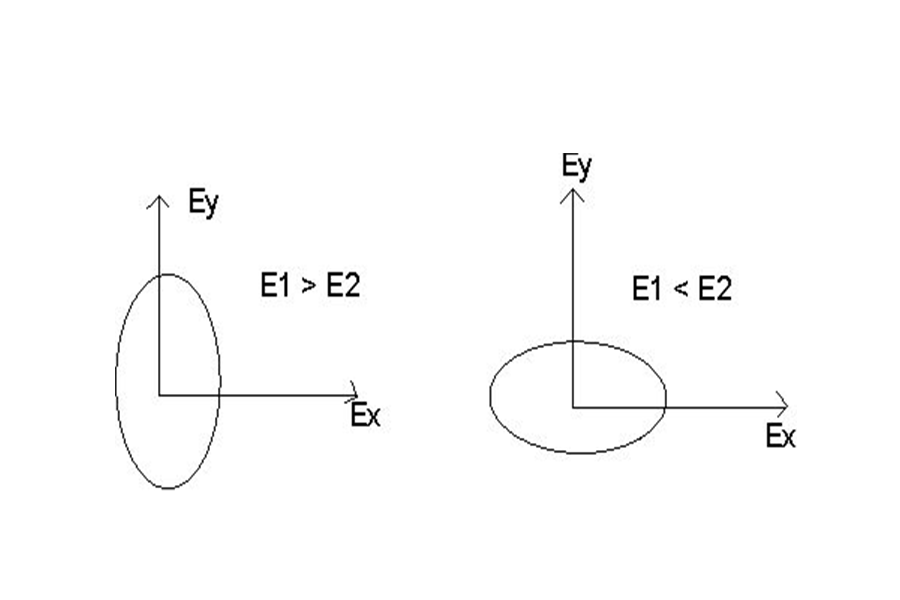
\includegraphics[width=.8\linewidth]{./graphics/eeee}
\caption{electric field vector}
\end{figure}

In practice,the application of the polarization shows how one state of polarization has advantage over another state of polarization.
\begin{figure}[h]
\centering
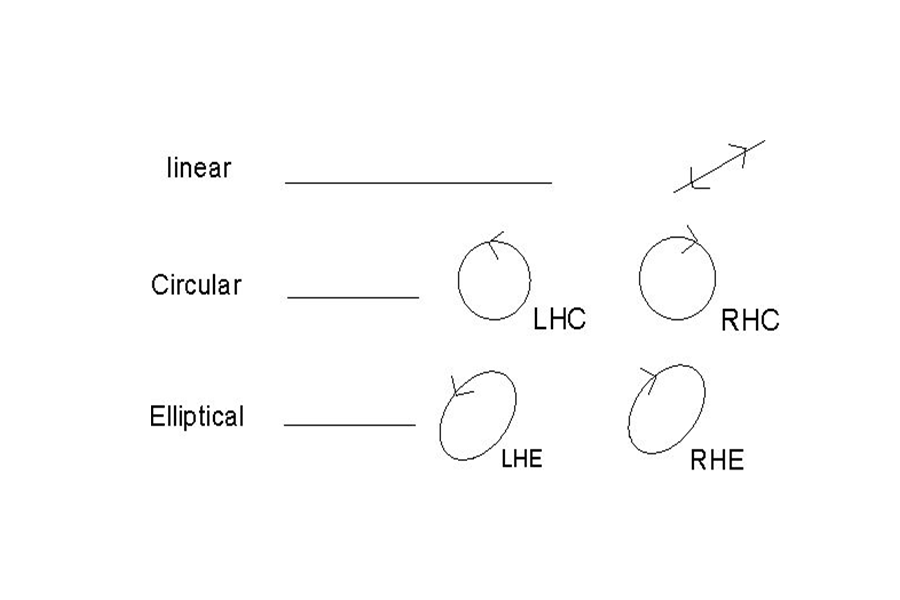
\includegraphics[width=.8\linewidth]{./graphics/eee}
\caption{state of polarization summary}
\end{figure}

So now if we define analytically certain parameters of the ellipse, we can actually capture the parameters of what is called Wave Polarization. Therefore characterizing the parameters of an ellipse, will correspond to a state of polarization.

Generally, there are two defining parameter of the ellipse;
\begin{enumerate}[(i)]
\item What is the orientation of the ellipse with respect to x-axis 
\item What is the ratio of the major and minor axis.
\end{enumerate}
If these two parameters are known, the ellipse can be specifically defined.
\begin{figure}[h]
\centering
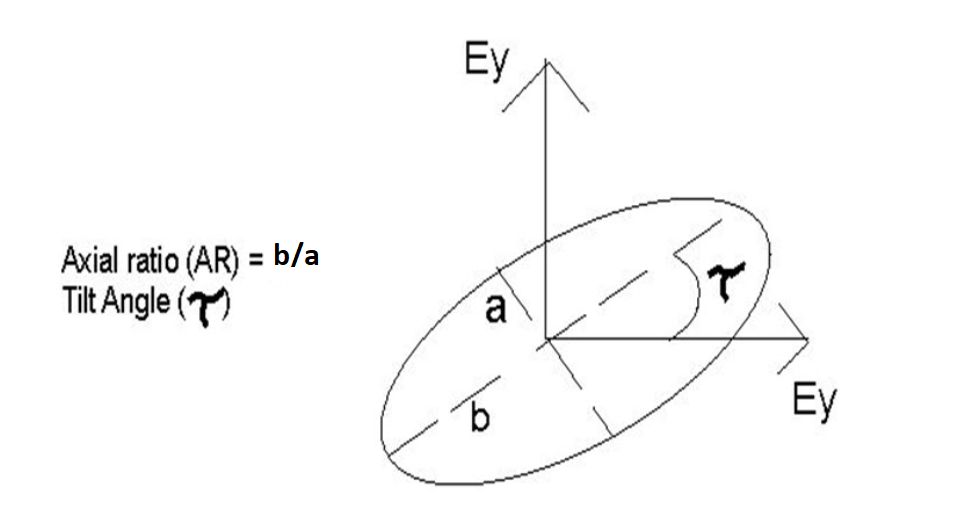
\includegraphics[width=1\linewidth]{./graphics/back}
\caption{ellipse parameters}
\end{figure}

\begin{center}
Axial Ratio (AR) = $\frac{a}{b}$\\
Tilt Angle ($\tau$)
\end{center}
AR can range from 1 to infinity.\begin{center}
1 $\leq $ AR $\leq $ $\infty $
\end{center}
If AR is equal to 1, that gives us Circular Polarization\\
If AR is equal to $\infty$, that gives us Linear Polarization\\
The range of $\tau $ is from $0^{o}$ to $180^{o}$ 
\begin{center}
$0^{o}$ $\leq $ $\tau $ $\leq $ $180^{o} $
\end{center}
*AR and $\tau $ define only the shape of the ellipse.To then capture the way the shape is drawn we assign a sign to AR;i.e if AR is positive, the sense of rotation is left handed, and if the AR is negative the sense of rotation is right handed.\\
Convention:
\begin{center}
If AR is +ve $\quad$ LH\\
If AR is -ve $\quad$ RH
\end{center}
*Now the complete description of the State of Polarization can be given by $\pm AR$ and $\tau $. These two parameters can be paired to specifically describe the State of Polarization.Also going back to the electric field we have two paired parameters that can also specifically describe the Sate of Polarization; i.e the ratio of $ E_2 $ and $ E_1 $, and $\delta$.

The State of Polarization can now be defined in two ways and they are equivalent, we have;
\begin{enumerate}[(i)]
\item In terms of the Electrical parameters, $\frac{E_1}{E_2}$ and $\pm \delta $.
\item In terms of the wave parameters, $\pm AR $ and $\tau $
\end{enumerate}
We require these two domain parameters because, many times we will like to generate the state of polarization, and we will like to know in what way this polarization should be generated by exciting two electrical fields that are horizontally and vertically polarized (i.e their amplitude and the phase difference $\delta $ between them), so we can generate the specific ellipse which was generated when the wave was launched.

So for generating a particular shape of ellipse or a particular wave of elliptical polarization, one should ask what parameters should be set electrically while generating the wave.

A relationship between the wave and electrical parameters will be required, also one can ask an analytical question (i.e for values of $\frac{E_1}{E_2} $ and $ \pm \delta $ what type of ellipse would be generated).

The values of $\frac{E_1}{E_2}$ and AR is a number, while the values of $\delta$ and $\tau $ is an angle. So for defining the state of polarization compactly, mathematicians have resulted to defining all the parameter in terms of angle (i.e $\gamma $ = $\tan^{-1} {\frac{E_1}{E_2}} $,$\epsilon $ =$ \cot^{-1} {\pm AR} $). 

In the next chapter we will see how compactly the State of Polarization is represented in terms of the pairs of angles and the conversion from one parameter to another, and how orthogonal state of polarization is generated.